\subsection{Portainer Configuration}\label{subsec:portainer-configuration}

\begin{flushleft}
    As mentioned in the Docker documentation, this container will make use of a volume named "portainer\_data", which
    will store the portainer data.
\end{flushleft}
\begin{flushleft}
    Also, to provide this container access to the docker management, we need to bind the file "/var/wun/docker.sock"
    to the docker container.
\end{flushleft}

\subsection{Adminer Configuration}\label{subsec:adminer-configuration}
\begin{flushleft}
    There is no configuration done to this package.
\end{flushleft}
\subsection{PHP Configuration}\label{subsec:PHH-configuration}
\begin{flushleft}
    As mentioned in the docker documentation, this container has been configured to have the PDO extension enabled.
\end{flushleft}
\subsection{Nginx Configuration}\label{subsec:nginx-configuration}

\begin{flushleft}
    To improve the security and having a better image through the client, this page uses SSL connections.
\end{flushleft}

\begin{flushleft}
    Since we have SSL connections, instead of restrict the access to the port 80, we made a simple forward from port 80
    to port 443, that wat we force the client to use the SSL protocol
\end{flushleft}
\lstinputlisting[language=C,label={lst:defaultConfigNginx}]{../config/nginx/default.conf}
\begin{flushleft}
    To improve the performance, we have enabled HTTP2.
    As mentioned before, we are using an SSL connection, so we needed to specify the certificate path.
    Also, to as a security measure, the logs been enabled, which we will store in a docker volume.
    Finally, since we are using a container without PHP itself, we need to enable a connection, so the Nginx server sends
    the connections to the PHP container in order to be executed.
\end{flushleft}
\lstinputlisting[language=C,label={lst:defaultWebNginx}]{../config/nginx/web.conf}

\subsection{PostgreSQL Configuration}\label{subsec:postgresql-configuration}
\begin{flushleft}
    Currently, the database contains 2 databases.
    \begin{itemize}
        \item contact\_form
        \item shop
    \end{itemize}
    As a security feature, the login either by local or remote host, have enabled "SCRAM-SHA-256".
\end{flushleft}
\subsubsection[Contact database structure]{Contact database structure}
\begin{flushleft}
    As the name hints, this database is used to store the contact forms received using the contact page from the website.
    Yet, the database consists of one table.
\end{flushleft}

\begin{center}
    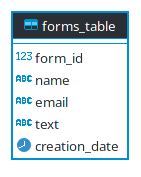
\includegraphics[scale=0.6]{DB_Table_Schema_Contact_FormV1}
\end{center}
\begin{center}
    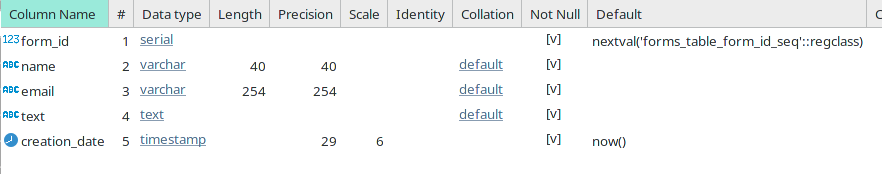
\includegraphics[scale=0.6]{DB_Table_Table_Contact_Form}
\end{center}

\begin{flushleft}
    As the name hints, this database is used to store the contact forms received using the contact page from the website.
    Yet, the database consists of one table.
\end{flushleft}
\begin{flushleft}
    It also contains a procedure called "insert\_form", which given the next information "\textit{(p\_name varchar,
    p\_email varchar, p\_text text)}", checks if the values are valid and in case of not being valid, will rise an error
    (more information in the Regex and Error List threads).
\end{flushleft}
\begin{flushleft}
    As a security measure, there been a user implemented using the next query:
    \lstinputlisting[language=SQL,label={lst:lstlisting}]{../Dockerfiles/postgresql/sources/contact_form_users.sql}
\end{flushleft}
\begin{flushleft}
    Taking a look at the query, we can observe that the first step is to revoke all the permissions in the database,
    that way we can ensure that all the users are limited to the options that we specifically gave.
\end{flushleft}


\newpage
\subsubsection[Shop database structure]{Shop database structure}
\begin{center}
%    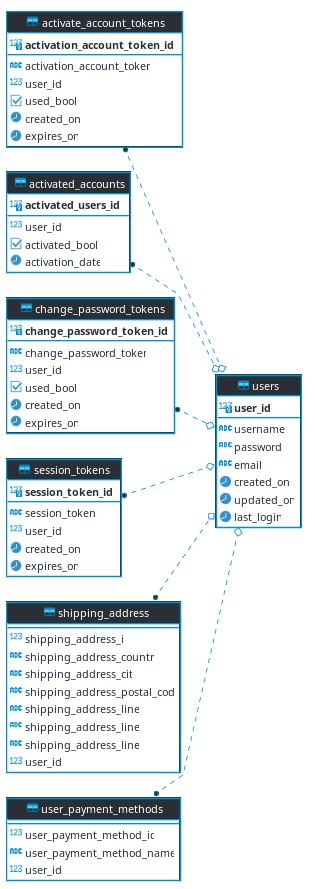
\includegraphics[scale=0.6]{DB_Table_Schema_ShopV1}
    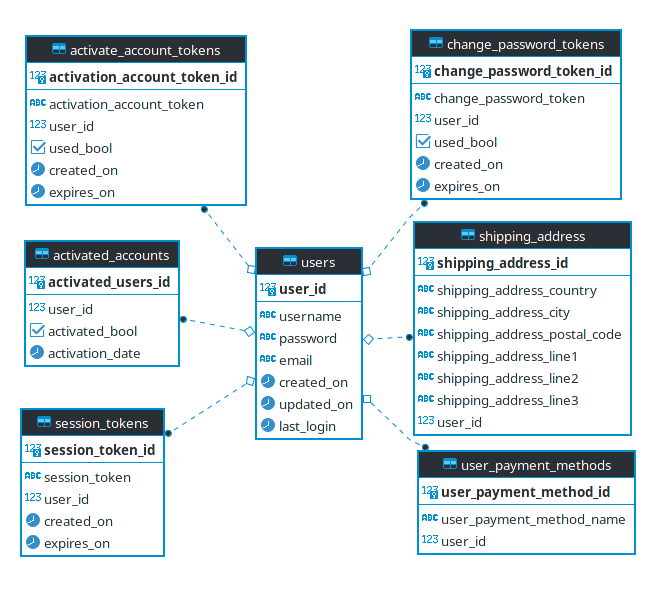
\includegraphics[scale=0.6]{DB_Table_Schema_ShopV4}
\end{center}
\begin{flushleft}
    Taking a look at the graph we can see how all the tables has a relation with the users table, bind by its user id.
    If we took a look at the queries used to create the tables, we could see how all would get deleted on cascade in case
    that the user was deleted.
    \url{https://github.com/OriolFilter/filterweb/blob/master/Dockerfiles/postgresql/sources/shop_skel.sql}
\end{flushleft}


\subsubsection[Plugins enabled]{Plugins enabled}
\begin{lstlisting}[language=SQL,label={lst:pgcrypto_enabling}]
CREATE EXTENSION if not exists pgcrypto;
\end{lstlisting}
\begin{flushleft}
    Pgcrypto was enabled in order to hash and salt the passwords, so the use critical information can be stored "securely".
\end{flushleft}

\newpage
\subsubsection[Data structure]{Data structure}
\begin{flushleft}
    \begin{itemize}
        \item Serial data (\_id values)
        \begin{itemize}
            \item Used to store data avoiding collisions while providing an identification point for the entry (used as a Primary Key).
        \end{itemize}
        \item Username
            \begin{itemize}
                \item Varchar of 20 length, still, it could be any length, even text, since how postgresql reserves memory,
                but in order to avoid issues during interactions with other applications, or, to facilitate upgrading to
                another Database System in the future (if it's needed), it's better to keep it sort of short.
                \begin{flushleft}
                    Usernames are checked by the next function: "function\_check\_user\_exists" returning a boolean, or
                    procedure "proc\_check\_user\_exists" raising an error in case the username already exists.
                \end{flushleft}
            \end{itemize}
        \item Password
        \begin{itemize}
            \item Varchar of 60 length since it's the length of a hashed value.
            \begin{flushleft}
                Passwords are hashed and use salt 8, while not providing any word to salt the value, being this one "randomized".
            \end{flushleft}
        \end{itemize}
        \item Email
        \begin{itemize}
            \item Varchar of 255 length since according to the next post, emails are actually unable to overcome that length.
            If in the future that changed, it could be easily modified.
            \begin{flushleft}
                \url{https://stackoverflow.com/questions/386294/what-is-the-maximum-length-of-a-valid-email-address}
            \end{flushleft}
        \end{itemize}
        \item created\_on - updated\_on - last\_login
        \begin{itemize}
            \item Stores a time stamp.
        \end{itemize}
        \item expires\_on
        \begin{itemize}

            \item Also stores a time stamp, but this one will also be used to check if the token for something (its function
            might depend on of which table is stored).
            By default  it's +30 minutes from its creation.
            \begin{flushleft}
            Used to check:
                \begin{itemize}
                    \item Login session is valid
                    \item Activate account token is valid
                    \item Update/Change password token is valid
                \end{itemize}
            \end{flushleft}
        \end{itemize}
        \item \_token values / varchar (200)
        \begin{itemize}
            \item Used to store randomized tokens.
            Like in the username or email fields, the value could ve easily modified if it was needed in the future.
        \end{itemize}
        \item shipping / payment methods data
        \begin{itemize}
            \item Mainly stored as a varchar, the length might vary depending on of the needs.
        \end{itemize}
    \end{itemize}
\end{flushleft}

\newpage
\subsubsection[Main functions]{Main functions}
\begin{flushleft}
    Like posteriorly will be shown with the error codes, postgresql it's intended to "break" (generate an error), in
    case something goes wrong.
    So it's mainly formed by procedures instead of functions, unless it's specifically required.

    \begin{itemize}
        \item  function return\_crypted\_pass(v\_txt varchar)
        \begin{itemize}
            \item Returns the hashed + salted (8) password using the function "crypt" (module "pgcrypto").
        \end{itemize}
        \item  procedure register\_user
        \begin{itemize}
            \item Registers the user with the values given, before inserting the values, checks that the values are valid.
        \end{itemize}
        \item  proc\_login\_session\_token
        \begin{itemize}
            \item Checks the given session token is valid, in case of being valid will enlarge its session 30 minutes from the moment,
            its used when the user loads a page.
        \end{itemize}
    \end{itemize}
\end{flushleft}


\newpage
\subsection{Data Validation}\label{subsec:data-validation}
\subsubsection[Regex]{Regex}

\begin{lstlisting}[language=yaml,label={lst:regexListing}]
PHP & JS:
    Registration:
        username: "^[a-zA-Z0-9_.+]{6,20}$"
        password: "^[a-zA-Z0-9$%.,?!@+_=-]{6,20}$"
        email:    "^[a-zA-Z0-9.!#$%&'*+/=?^_`{|}~-]+@[a-zA-Z10-9-]+\.+[a-zA-Z0-9-]+$"

    Contact form:
        name:  "^[\w0-9 ]{4,40}$"
        email: "^[a-zA-Z0-9.!#$%&'*+/=?^_`{|}~-]+@[a-zA-Z10-9-]+\.+[a-zA-Z0-9-]+$"
        text:  "^[\w\W]{20,255}$"

    Change password form:
        token: "^[a-zA-Z0-9]{60}$"

    Payment methods:
        name: '^[a-zA-Z0-9 ]{6,20}$'
        id: '^[0-9]+$'
    Shipping adress:
        Country code: '/^[a-zA-Z]{2}$/'
        id: '/^[0-9]+$/'
        postal code & city: '/^[\w\W]+$/' # Checks not empty
        address line 1: '/^[\w\W]{5,200}$/'
        address line 2 & 3 : "/^[\w\W]*$/" # A lie, doesn't checks nothing

POSTGRESQL:
    Contact form:
        name:  "^[\w0-9 ]{4,40}$"
        email: "^[a-zA-Z0-9.!#$%&'*+=?^_`{|}~-]+@[a-zA-Z10-9-]+\.[a-zA-Z0-9-]+$"
\end{lstlisting}

\subsubsection[Javascript]{Javascript}

\begin{flushleft}
    Uses Regex and default java functions in order to check if the fields are valid, yet it doesn't really look at specific stuff.
\end{flushleft}

\begin{flushleft}
    Uses Ajax when receiving a response from the server, so can format a response for the user.
\end{flushleft}

\subsubsection[PostgreSQL]{PostgreSQL}

\begin{flushleft}
    Uses functions and procedures in order to detect errors, alongside with Regex.
\end{flushleft}

\subsubsection[PHP]{PHP}
\begin{flushleft}
    Uses functions and procedures in order to detect errors, alongside with Regex.
    PHP uses the errors captured to form a response for the client.
\end{flushleft}

\subsection{Error Thread}\label{subsec:error-thread}
\subsubsection{Notes}\label{subsubsec:notes}
\begin{flushleft}
    The errors are supposed to be handled by something, but not by postgresql (unless it's something specific), since
    there is no need of rollback/commit, due postgresql nature, that controls this automatically.
\end{flushleft}
\begin{flushleft}
    PHP and JavaScript uses these errors to format responses for the client based in the code received.
\end{flushleft}

\subsubsection{Error Codes}\label{subsubsec:error-codes}
\begin{lstlisting}[language=yaml,label={lst:errorListing}]
php & js:
    '0': 'Unknown error',

    '1': 'Success',

    '2': 'Missing field(s)',
    '2.1': 'Username field is missing',
    '2.2': 'Password field is missing',
    '2.3': 'Email field is missing',
    '2.4': 'Repeat password field is missing',
    '2.5': 'Repeat email field is missing',
    '2.6': 'Name field is missing',
    '2.7': 'Text field is missing',
    '2.8': 'Payment method name field is missing',
    '2.9': 'Payment method info field is missing',
    '2.10': 'Payment method id field is missing',
    '2.11': 'Shipping address fields topic',
    '2.11.1': 'Shipping address country field is missing',
    '2.11.2': 'Shipping address city field is missing',
    '2.11.3': 'Shipping address postal code field is missing',
    '2.11.4': 'Shipping address line 1 field is missing',
    '2.11.5': 'Shipping address id field is missing',

    '3': 'Requirements not achieved',
    '3.1': 'Username does not meet the requirements',
    '3.2': 'Password does not meet the requirements',
    '3.3': 'Email does not meet the requirements',
    '3.4': 'Name does not meet the requirements',
    '3.5': 'Text does not meet the requirements',
    '3.6': 'Payment method name does not meet the requirements',
    '3.7': 'Payment method info does not meet the requirements',
    '3.8': 'Payment method id does not meet the requirements', # It's a numeric value only
    '3.9': 'Shipping address fields topic',
    '3.9.1': 'Shipping address country field does not meet the requirements',
    '3.9.2': 'Shipping address city field does not meet the requirements',
    '3.9.3': 'Shipping address postal code field does not meet the requirements',
    '3.9.4': 'Shipping address line 1 field does not meet the requirements',
    '3.9.5': 'Shipping address line 2 field does not meet the requirements',
    '3.9.6': 'Shipping address line 3 field does not meet the requirements',
    '3.9.7': 'Shipping address id does not meet the requirements', # It's a numeric value only

    '4': 'Field matching',
    '4.1': 'Passwords don\'t match',
    '4.2': 'Emails don\'t match',

    '5': 'Client-Server errors',
    '5.1': 'There was a unknown error sending the data, please, try again bit later, if this error is consistent please contact an administrator.',
    '5.2': 'Server under maintenance, please, try again bit later.'

    '6': 'Database side error'
    '6.1': 'Data Insert errors',
    '6.1.1': 'Username is already exists',
    '6.1.2': 'Email is already exists',

    '6.2': 'Data Select errors',
    '6.2.1': 'Username not found',
    '6.2.2': 'User_id not found',
    '6.2.3': 'Email not found',
    '6.2.4': 'Token not found',
    '6.2.5': 'Payment method not found',
    '6.2.6': 'Shipping address not found',

    '6.3': 'Tokens',
    '6.3.1': 'Token not valid',
    '6.3.2': 'Token already used',
    '6.3.3': 'Token expired',
    '6.3.4': 'Token is null or empty',

    '6.4': 'Database connection error',
    '6.4.1': 'Error communicating to database',
    '6.4.2': 'Wrong credentials connecting to database',
    '6.4.3': 'The user don\'t has permission for the requested action(s)',

    '6.5': 'Functions error',
    '6.5.1': 'Error generating token',


    '7': 'Account related issues',
    '7.1': 'The account is not activated',
    '7.2': 'The account is already activated',
    '7.3': 'The account been banned',

    '8': 'PHP mailer issues',
    '8.1': 'Email couldn\'t be send',
    '8.2': 'Email address is missing',
    '8.3': 'Body is missing',
    '8.4': 'Subject is missing',

    '9': 'Invalid Credentials',

    '10': 'Product stuff',

    '11': 'User conf stuff',

    '11.2': 'Not valid payment method data'

    '12': 'Order Stuff'
postgresql:
  - 'Due postgresql not being able to use the same syntax as php and since the error codes seems easy to read using the syntax already done, it's been decided to leave the php and js codes as they, while using a similar (but valid) syntax for postgresql.'
  - 'P0000'
  - 'P + first number + second number +  last number'
  examples:
    - '7     :P7000'
    - '8.3   :P8300'
    - '6.4.4 :P6404'
    - '2.1   :P2100'
    - '2.10  :P2010'
\end{lstlisting}
